\documentclass[amsmath,amssymb,12pt,eqsecnum]{revtex4}
\usepackage{ graphicx, amsmath, amsmath, amssymb, subfigure}
 
\newcommand{\vphi}[0]{\delta\phi}
\newcommand{\lpa}[0]{\lp A}
\newcommand{\dlg}[0]{\lp g}

\newcommand{\depg}[0]{\ep g}
\newcommand{\virt}[0]{\hat{\delta}}
\newcommand{\Dvphi}[1]{\nabla_{#1}\vphi}
\newcommand{\DDvphi}[2]{\nabla_{#1}\nabla_{#2}\vphi}

\newcommand{\Dvvphi}[1]{\nabla_{#1}\virt\vphi}
\newcommand{\DDvvphi}[2]{\nabla_{#1}\nabla_{#2}\virt\vphi}

\newcommand{\tmat}[4]{\bigg( \begin{array}{cc} #1 & #2 \\ #3 & #4 \end{array}\bigg)}
\newcommand{\expec}[1]{\left\langle #1\right\rangle}
\newcommand{\half}[0]{\frac{1}{2}}
\newcommand{\cs}[3]{\Gamma^{#1}_{\,\,\,\, #2#3}}

\newcommand{\pd}[2]{\frac{\partial #1}{\partial #2}}
\newcommand{\ld}[0]{\mathcal{L}}
\newcommand{\md}[0]{\mathcal{M}}
\newcommand{\dd}[0]{\textrm{d}}
\newcommand{\defn}[0]{\equiv}
\newcommand{\diag}[0]{\textrm{diag}}
\newcommand{\qsubrm}[2]{{#1}_{\scriptscriptstyle{\textrm{#2}}}}

\newcommand{\subsm}[2]{{#1}_{\scriptscriptstyle{#2}}}
\newcommand{\supsm}[2]{{#1}^{\scriptscriptstyle{#2}}}
\newcommand{\qsuprm}[2]{{#1}^{\scriptscriptstyle\textrm{#2}}}
\newcommand{\subpsm}[3]{\subsm{#1}{#2}^{\scriptscriptstyle #3}}
 

\newcommand{\symmb}[0]{\varrho}
\newcommand{\AW}[0]{A_{\mathcal{W}}}
\newcommand{\BW}[0]{B_{\mathcal{W}}}
\newcommand{\CW}[0]{C_{\mathcal{W}}}
\newcommand{\DW}[0]{D_{\mathcal{W}}}
\newcommand{\EW}[0]{E_{\mathcal{W}}}

\newcommand{\AP}[0]{A_{\mathcal{P}}}
\newcommand{\BP}[0]{B_{\mathcal{P}}}
\newcommand{\CP}[0]{C_{\mathcal{P}}}
\newcommand{\DP}[0]{D_{\mathcal{P}}}
\newcommand{\EP}[0]{E_{\mathcal{P}}}
\newcommand{\FP}[0]{F_{\mathcal{P}}}
\newcommand{\GP}[0]{G_{\mathcal{P}}}

\newcommand{\sol}[0]{\ld_{\scriptscriptstyle\{2\}}}

\newcommand{\lcdm}[0]{$\Lambda$CDM}

\newcommand{\coup}[0]{\mathcal{Q}}
\newcommand{\vmkin}[0]{\mathcal{K}}

\newcommand{\pis}[0]{ {\Pi}^{\scriptscriptstyle\rm{S}}}
\newcommand{\xis}[0]{ {\xi}^{\scriptscriptstyle\rm{S}}}
\newcommand{\xisdot}[0]{ {\dot{\xi}}^{\scriptscriptstyle\rm{S}}}
 
\newcommand{\nphiu}[1]{\nabla^{#1}\phi}
\newcommand{\nphid}[1]{\nabla_{#1}\phi}

\newcommand{\gbm}[1]{\bm{#1}}
\newcommand{\rbm}[1]{{\bf{#1}}}
\newcommand{\ci}[0]{\textrm{i}}
 \newcommand{\kin}[0]{{\mathcal{X}}}
\newcommand{\hct}[0]{\mathcal{H}}
\renewcommand{\figurename}{Figure}
\newcommand{\ep}[0]{{ {\delta}_{\scriptscriptstyle{\rm{E}}}}}
\newcommand{\lp}[0]{{ {\delta}_{\scriptscriptstyle{\rm{L}}}}}
\def\be{\begin{equation}}
\def\ee{\end{equation}}
\def\bea{\begin{eqnarray}}
\def\eea{\end{eqnarray}}
\def\bse{\begin{subequations}}
\def\ese{\end{subequations}}
\newcommand{\lied}[1]{\pounds_{#1}}
\newcommand{\spnab}[0]{{\overline{\nabla}}{}}



%\renewcommand{\vphi}{\varphi}

\newcommand{\sech}[0]{\textrm{ sech}}
\newcommand{\fref}[1]{{Figure \ref{#1}}}
\newcommand{\tref}[1]{{Table \ref{#1}}}
\newcommand{\secref}[1]{{section \ref{#1}}}
\newcommand{\Secref}[1]{{Section \ref{#1}}}
% PUT CATCH ON THE END OF SQUARE-ROOT SYMBOLS
\newcommand{\rsbb}[2]{#1_{\mathbb{#2}}}

\newcommand{\dg}[0]{\delta g}
\let\oldsqrt\sqrt
% it defines the new \sqrt in terms of the old one
\def\sqrt{\mathpalette\DHLhksqrt}
\def\DHLhksqrt#1#2{%
\setbox0=\hbox{$#1\oldsqrt{#2\,}$}\dimen0=\ht0
\advance\dimen0-0.2\ht0
\setbox2=\hbox{\vrule height\ht0 depth -\dimen0}%
{\box0\lower0.4pt\box2}}
 
 
 \newcommand{\Af}[0]{\mathsf{A}}
\newcommand{\Bf}[0]{\mathsf{B}}
\newcommand{\Cf}[0]{\mathsf{C}}
\newcommand{\Df}[0]{\mathsf{D}}
\newcommand{\Ef}[0]{\mathsf{E}}
\newcommand{\comment}[1]{{\color{red}[#1]}}
\newcommand{\note}[1]{{\color{blue}#1}}
\newcommand{\todo}[1]{{\color{blue}#1}}
\newcommand{\Mpsq}[0]{{\qsubrm{M}{pl}^2}}
\usepackage[breaklinks, colorlinks, citecolor=blue]{hyperref}
\linespread{1}
\begin{document}

 

\title{Integrating the sequestering equations of motion}
\author{Jonathan A. Pearson}
\email{j.pearson@nottingham.ac.uk}
\affiliation{School of Physics \& Astronomy, University of Nottingham, Nottingham, NG7 2RD, U.K.}

\date{\today}


\begin{abstract} 
In conversation with Adam Moss, Tony Padilla, Nemanja Kaloper.

\end{abstract}

\maketitle
\section{Introduction}
We use the $\phi$-gauge. See \cite{Kaloper:2013zca, Kaloper:2014dqa, Kaloper:2014fca} and \cite{Avelino:2014nqa, Avelino:2014aea, Kluson:2014tma}.  The equations of motion in spatially flat FRW space-time are
\bse
\label{frw-eqnsofmotion}
\bea
3\Mpsq H^2 = \qsubrm{\rho}{m} + \half \dot{\phi}^2 + \qsubrm{m}{slope}^3\phi,
\eea
\bea
3\Mpsq \dot{H} = - \frac{3}{2}\left( \qsubrm{\rho}{m} + \qsubrm{p}{m} + \dot{\phi}^2\right),
\eea
\bea
\ddot{\phi} + 3 H \dot{\phi} + \qsubrm{m}{slope}^3=0,
\eea
\ese
and are subject to the constraint
\bea
\label{eq:seq_constraint}
\langle\dot{\phi}^2\rangle - 4\qsubrm{m}{slope}^3 \expec{\phi} + \expec{3\qsubrm{p}{m} - \qsubrm{\rho}{m}} = 0.
\eea
The symbol $\expec{Q}$ is defined as the historic integral; in the FRW background this is
\bea
\expec{Q} \defn \frac{\int_{\qsubrm{t}{bang}}^{\qsubrm{t}{crunch}} \dd t \,a(t)^3\, Q(t)}{\int_{\qsubrm{t}{bang}}^{\qsubrm{t}{crunch}} \dd t\, a(t)^3}.
\eea
Note that the start-point of the integrals is the ``big bang'', and the end-point is the ``big-crunch''. The dark energy theory considered here is guaranteed to have a crunch-ending.
The subscript ``m'' denotes {\it all} matter quantities (e.g., CDM and radiation).

The $\phi$-gauge condition requires that $\expec{{T^{\mu}}_{\nu}}=0$. From the field equation, this means that the historic average of the Ricci scalar must vanish:
\bea
\label{eq:vanish_R}
\expec{R} = 0.
\eea
The constraint (\ref{eq:seq_constraint}) is equivalent to (\ref{eq:vanish_R}).

\section{Methods of solving}
Solving the equations of motion (\ref{frw-eqnsofmotion}) is ``easy'' (for example, see the  {\tt deevolve} code I've written with J. Bloomfield). However, the constraint (\ref{eq:seq_constraint}) does not have an obvious implementation strategy. 
%\subsection{Re-writing}
%Can the equations of motion be re-written to automatically satisfy (\ref{eq:seq_constraint})?  We have in mind ``constrained field-theory'' problems whereby a given set of boundary conditions and some conserved quantity (like charge, or winding number) is used to obtain the field configurations for solitons. These are done by writing down an energy functional and obtaining the field configurations which minimize the energy with a given value of (for example) charge. Here, we are interested in field configurations which minimise the action, with a given value of ``constraint''.
\subsection{MCMC method}
An MCMC method may work: for a given set  of ``parameters'',
\bea
\mathcal{P}= \left\{ \mbox{inital conditions}, \mbox{model parameters}\right\},
\eea
we could evolve the equations of motion (\ref{frw-eqnsofmotion}), and then compute the value of 
\bea
\mathcal{C} \defn \langle\dot{\phi}^2\rangle - 4\qsubrm{m}{slope}^3 \expec{\phi} + \expec{3\qsubrm{p}{m} - \qsubrm{\rho}{m}}.
\eea
This would populate the space $\mathcal{P}$ with values of $\mathcal{C}$; those which are compatible with the sequestering scenario have $\mathcal{C}=0$. {\it If} there exists  some sensible measure on $\mathcal{P}$ which yields $|\mathcal{C}| \ll 1$ on some sub-manifold, then MCMC can be used to ``hone in on'' the sequestering-favoured regions of $\mathcal{P}$. Since we do not know the location of  seq-fav-regions, we will treat the entire space $\mathcal{P}$ with equality.

The MCMC engine would search the space $\mathcal{P}$ for regions which minimize $|\mathcal{C}|$. Finding the minimal regions is ``all this method could do''.
\section{Implementing into {\tt deevolve}}
We will use the {\tt deevolve} code to evolve the equations of motion -- the equations are evolved in conformal time. A given set of parameters (i.e., scalar field initial conditions, and cosmological parameters) are used to solve the equations of motion. We evolve untill the Universe collapses (i.e., $a=0$).

The action is
\bea
S = \qsubrm{m}{P}^2 \int \dd^4x\,\sqrt{-g}\left[ \half R + \hct_0^2 \left( - \frac{1}{2\hct^2_0}(\partial\phi)^2 - V(\phi) \right) \right] + \qsubrm{S}{m}[g_{\mu\nu}; \Psi]
\eea

The Ricci scalar in conformal time is given by
\bea
R = \frac{6}{a^2}\left( \dot{\hct} + \hct^2 + k^2\right).
\eea
Also, the measure in conformal time is
\bea
\sqrt{-g} = a(\tau)^4.
\eea 
The historic average in conformal time is
\bea
\expec{Q} \defn \frac{\int_{\qsubrm{\tau}{bang}}^{\qsubrm{\tau}{crunch}} \dd \tau \,a(\tau)^4\, Q(\tau)}{\int_{\qsubrm{\tau}{bang}}^{\qsubrm{\tau}{crunch}} \dd \tau\, a(\tau)^4}.
\eea
The crunch-time $\qsubrm{\tau}{crunch}$ is defined to be where $a\left(\qsubrm{\tau}{crunch}\right)=0$.

\section{Numerical solutions}
We have integrated the equations of motion (in conformal time), using {\tt deevolve}. The material content is: matter, radiation, and quintessence scalar field with linear potential (see, e.g., \cite{Kallosh:2003bq}). This yields a number of parameters used to parameterize the solutions: including $\qsubrm{\Omega}{m}, \qsubrm{\Omega}{r}$, the parameter $\qsubrm{m}{slope}$, and the initial values of the scalar $\phi_0, \dot{\phi}_0$. We note that at this stage ``solutions are obtained'' which are not necessarily sequestering. That is, the solutions to the equations of motion do not necessarily satisfy $\expec{R}=0$. In \fref{fig:evplots1} we plot the evolution of various quantities; the different lines correspond to different  initial values of the scalar field.

We will compute
\bea
C\left( \qsubrm{\tau}{max}\right) \defn \frac{\int_{\qsubrm{\tau}{start}}^{\qsubrm{\tau}{max}} \dd\tau\,a^4\,R}{\int_{\qsubrm{\tau}{start}}^{\qsubrm{\tau}{max}} \dd\tau\,a^4} = \expec{R}\left( \qsubrm{\tau}{max}\right),
\eea
and understand the convergence properties of $C\left( \qsubrm{\tau}{max}\right)$ as the ``crunch'' is approached. These are plotted in \fref{fig:num_solns_deevolve}.

\begin{figure}[!t]
      \begin{center}
{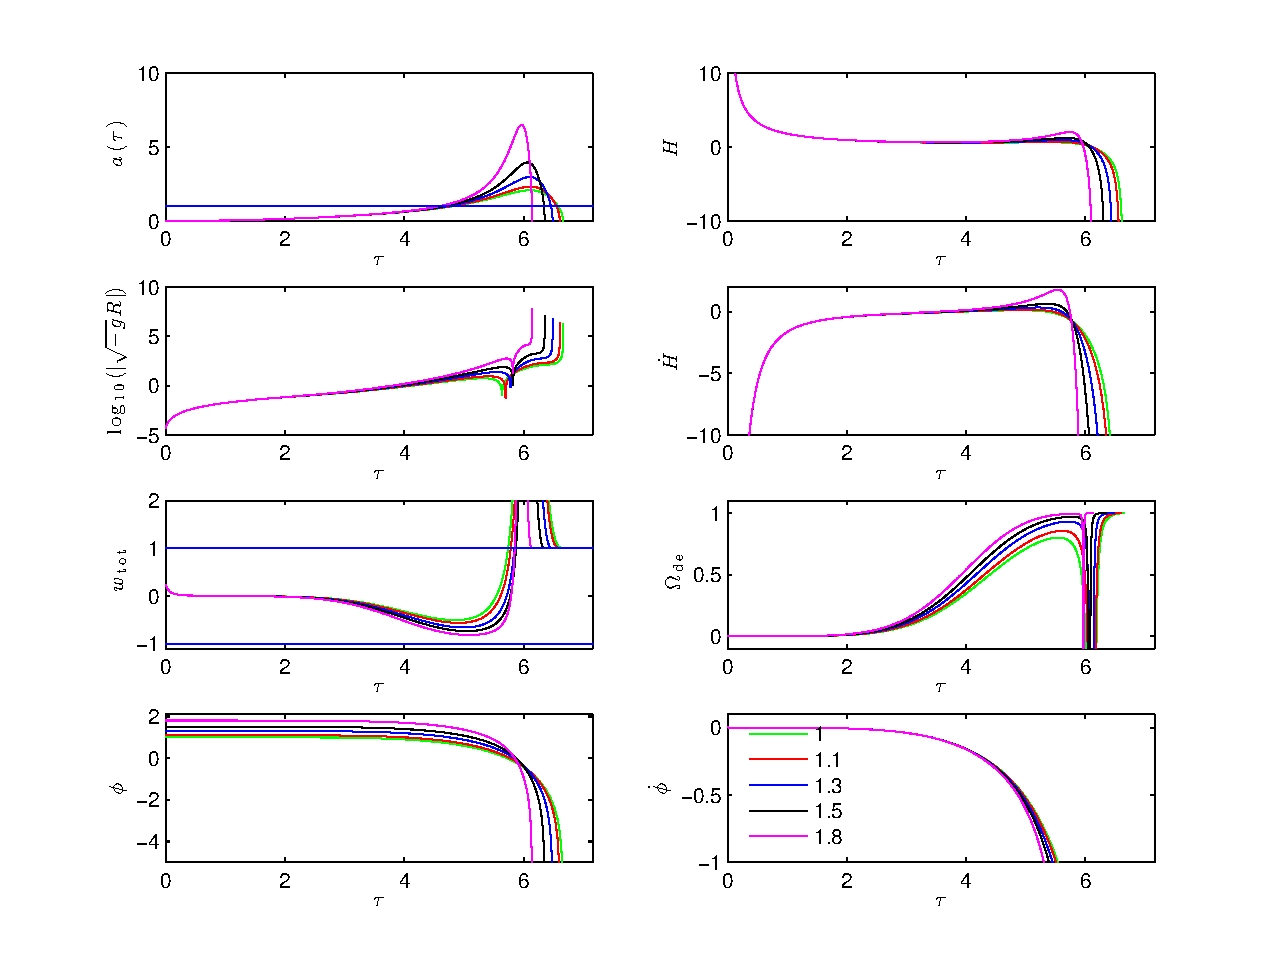
\includegraphics[scale=0.8]{images/evPlots.pdf}}
      \end{center}
\caption{The evolution of various quantities; each line corresponds to a different value of $\phi_0$, as shown in the legend. We have fixed $\dot{\phi}_0 = 0.01, \qsubrm{m}{slope} = 1$; all other cosmological parameters have values as given in the table -- note that these have zero spatial curvature. In the top right panel we show the evolution of the scale factor, $a(\tau)$: it is clear that these models describe expanding universes which then collapse (when $a=0$); we have drawn on a line at $a=1$, which corresponds to ``today''. It is also worth noting the total ``equation of state'' parameter, $\qsubrm{w}{tot}$ which we plot in the third plot down on the left. It shows that the scalar field acts like a ``stiff fluid'', with $w=1$ at the crunch.} \label{fig:evplots1}
\end{figure}

\begin{figure}[!t]
      \begin{center}
{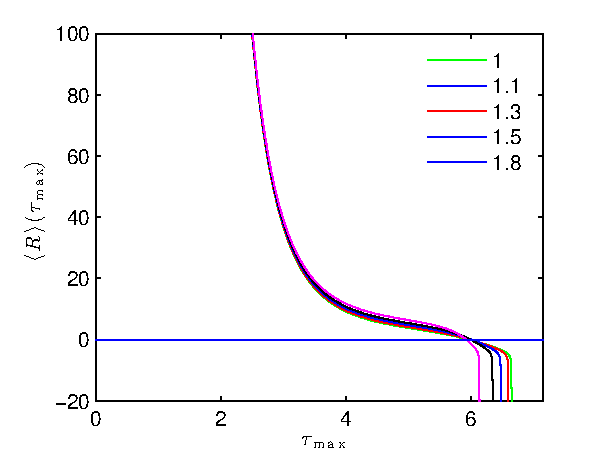
\includegraphics[scale=0.8]{images/Cplot.pdf}}
      \end{center}
\caption{Plot to enhance understanding of the convergence of the historic average, near the crunch singularity; each curve has identical parameter values to those in \fref{fig:evplots1}. It is clear that $\expec{R}$ has a zero for $\qsubrm{\tau}{max}\sim 6$, but it quickly becoms very negative as the crunch is approached. }\label{fig:num_solns_deevolve}
\end{figure}

{\renewcommand{\arraystretch}{1.4}
\begin{table}%[b] 
%\begin{andptabular}{X[4c]X[4c] }%
\begin{center}
\begin{tabular}{||c |  c ||}
%{Summary  of    commonly used symbols}
\hline
\textbf{Parameter} & \textbf{Fiducial value} \\
\hline
Hubble, $h$ ($H_0 = 100h$km/s/Mpc) & 0.7 \\\hline
Current matter fraction, $\qsubrm{\Omega}{m}h^2$ &0.137  \\\hline
Current baryon fraction, $\qsubrm{\Omega}{b}h^2$ &0.02240  \\\hline
Current curvature fraction, $\qsubrm{\Omega}{k}h^2$ &0.0 \\\hline
Effective rel.dofs, $\qsubrm{N}{eff}$ &3.046 \\\hline
Photon temperature, $T_{\gamma}$ & 2.72548 \\\hline
\end{tabular}\caption{Fiducial values of the parameters}\label{tab:fid_params}
\end{center}
\end{table}
}

\section{Constraints}
\subsection{Using {\tt deevolve}}
Note that {\tt deevolve} does not have nuisance parameters in the likelihood computation. \comment{Can we modify {\tt COSMOMC} to not run {\tt CAMB}?}

In \fref{fig:const_fixed_cosm_deevolve} we plot the constraints on the dark energy parameters -- note that these arent selected to be ``sequestering solutions''.
\begin{figure}[!t]
      \begin{center}
{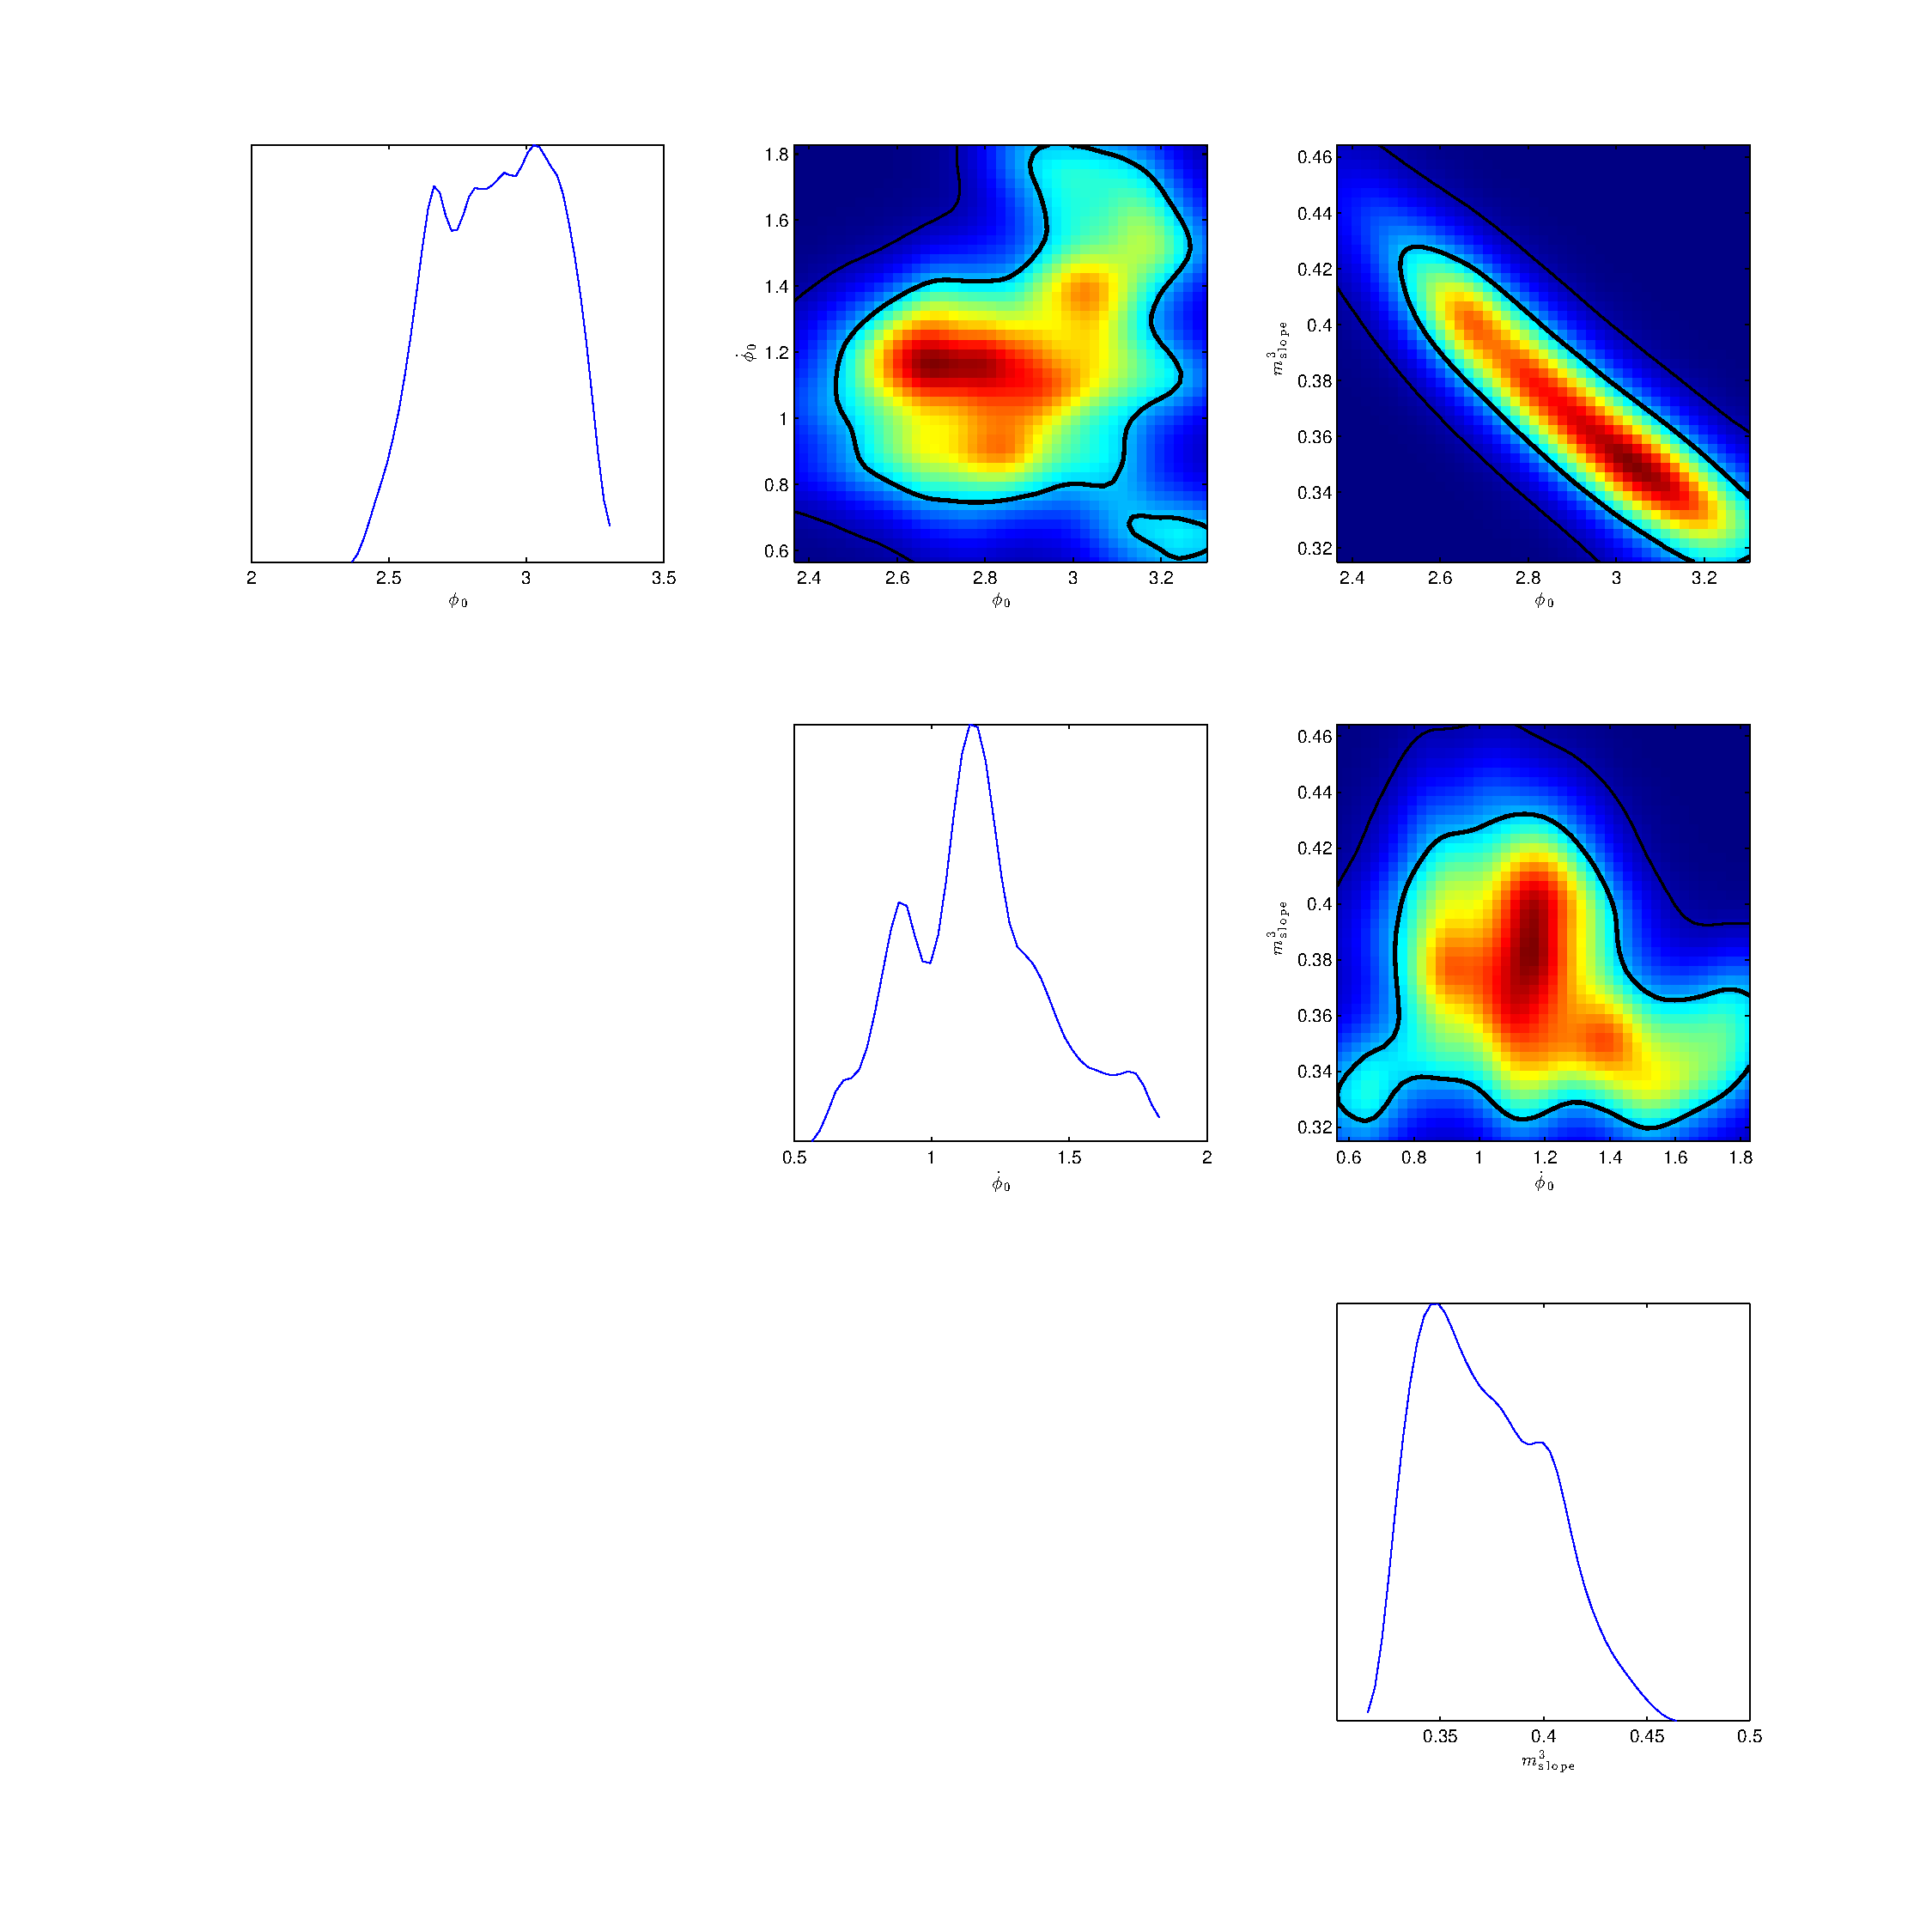
\includegraphics[scale=0.4]{images/tri_run_10000.pdf}}
      \end{center}
\caption{Constraints using WMAP+BAO+SN1a. All other cosmological parameters are held fixed to their fiducual values, just for simplicity. Also: these have not been selected to be ``sequestering'' solutions. }\label{fig:const_fixed_cosm_deevolve}
\end{figure}

\note{
\section{TO DO}
- Planck cut-off for $R$ \& testing sequestering solutions

\subsection{Finding sequestering solutions}
Suppose we have evolved the equations $\{\mathcal{E}\}$, for a given set of parameters $\{\mathcal{P},p\}$. This gives a value of the constraint, $C \defn \expec{R}$. We then want to find a new value of the parameter $p$ that goes toward minimizing the value of $C$. That is, we want to find the root of the function $C(p)$. We can do this with Newton-Raphson's method, which tells us how to pick the next value of the parameter, based on the current value of $C$ and its derivative,
\bea
p_{n+1} = p_n - \frac{C(p_n)}{C'(p_n)}.
\eea
We can approximate the derivative via finite differences,
\bea
C'(p_n) \approx \frac{C(p_n + \Delta) - C(p_n - \Delta)}{2\Delta}
\eea
}

\clearpage
\section{Solutions}
We have integrated the equations of motion, for a set of values of the mass $m^3$ and curvature $\qsubrm{\Omega}{k}h^2$ (all other parameters are set to their fiducial values). Results are given in \fref{fig:plots1}. It is apparent that the maximum size, and age, of the Universe is relatively unnaffected by the spatial curvature. All of these models give $w\approx -1$.


\begin{figure}[!t]
      \begin{center}
\subfigure[\, $\qsubrm{a}{max} $]{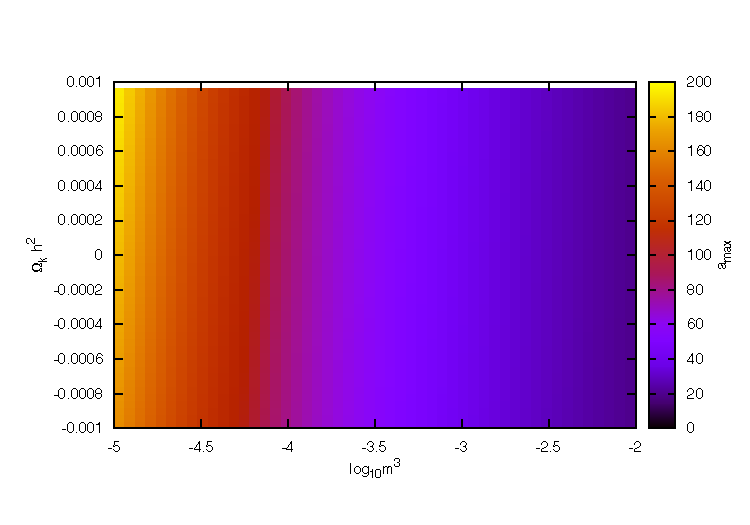
\includegraphics[scale=0.5]{images/sweep_test22_amax.pdf}}
\subfigure[\, $\qsubrm{t}{max} $]{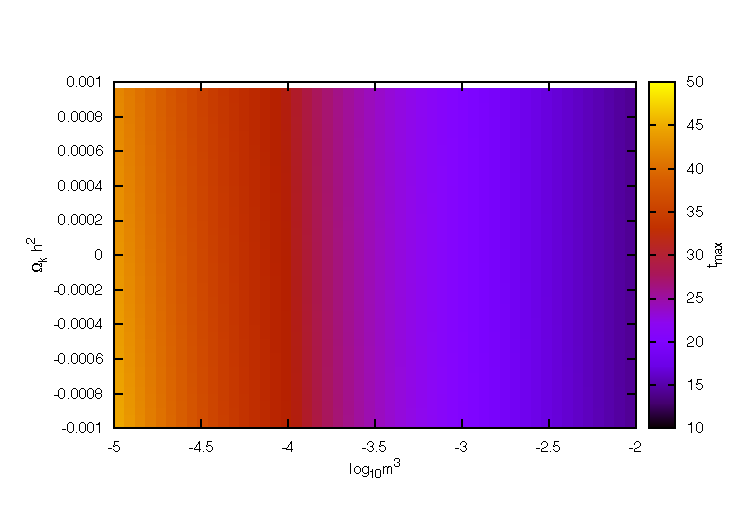
\includegraphics[scale=0.5]{images/sweep_test22_tmax.pdf}}
\subfigure[\, $10^3(1+w_0)$]{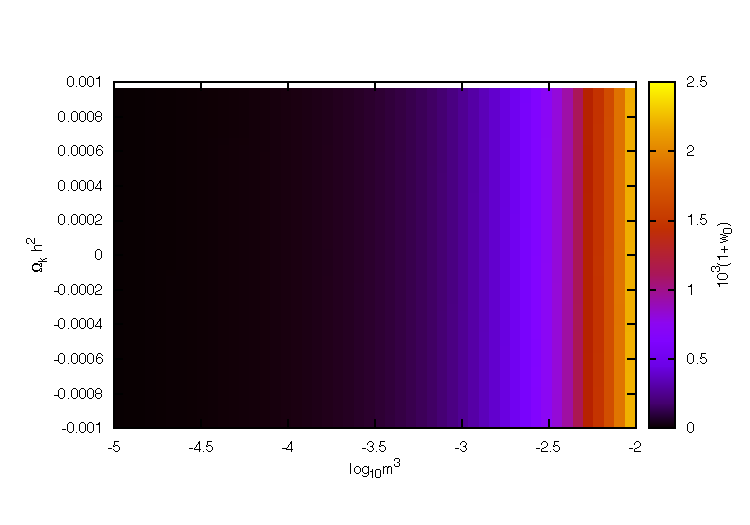
\includegraphics[scale=0.5]{images/sweep_test22_w0.pdf}}
\subfigure[\, $\log_{10}|\langle R\rangle|$]{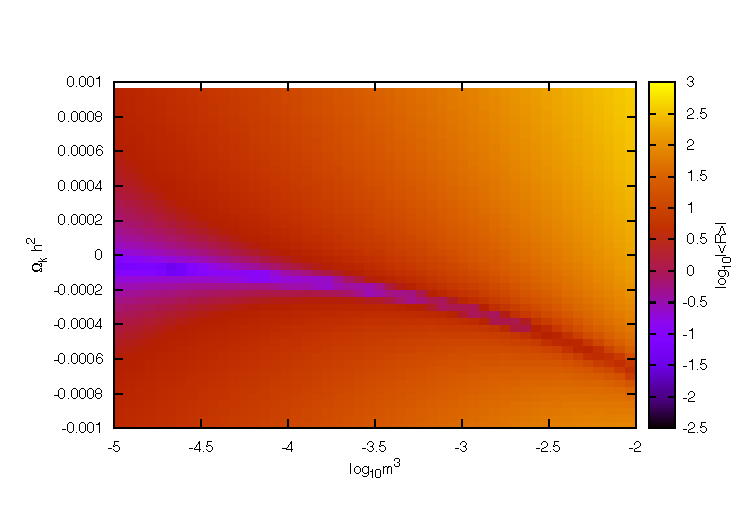
\includegraphics[scale=0.5]{images/sweep_test22.pdf}}
      \end{center}
\caption{ Various diagnostic quantities as functions of $m^3$ and the curvature $\qsubrm{\Omega}{k}h^2$. In (d) it is clear that there is some subset of the $(m^3, \qsubrm{\Omega}{k}h^2)$-space which naturally yields sequestering solutions: these are where $\langle R\rangle = 0$, and lie along the band which is apparent. We also note that for all of these models, the current value of the dark energy equation of state parameter, $w_0$, is very close to $-1$. In (a) we show that the smaller values of $m^3$ produce bigger Universes (before their inevitible collapse) -- these bigger Universes have total age given in (b). Note that the ''band'' of $\langle R\rangle = 0$ does not show up via any features in any of the plots in (a)-(c).}\label{fig:plots1}
\end{figure}

\bibliographystyle{JHEP}
\bibliography{refs}

\end{document}